\documentclass[12pt]{article}

\usepackage[margin=1in]{geometry}
\usepackage{xfrac}
\usepackage{graphicx}
\usepackage{amssymb}
\usepackage{amsmath}
\usepackage{xcolor}
\usepackage[colorlinks=true]{hyperref}
\usepackage{braket}
\usepackage{relsize}
\usepackage{palatino}
\usepackage{mathpazo}
\usepackage{xspace}
\usepackage{comment}
\usepackage{hyperref}
\newcommand{\degrees}{^{\circ}}
\newcommand{\titlecolor}{\bf \it \color{blue}}
\newcommand{\unit}[1]{\,\ensuremath{\mathrm{#1}}\xspace}

\usepackage{amsmath}
\usepackage{booktabs}
\usepackage{multirow}
\usepackage[final]{pdfpages}

\definecolor{Gray}{gray}{0.9}
\definecolor{LightCyan}{rgb}{0.88,1,1}
\definecolor{LightRed}{rgb}{1,0.92,0.92}
\newif\ifsol

%\soltrue % to show solutions
\solfalse % to hide solutions

\newcommand{\solColor}{blue}
\newcommand{\sol}[1]{\ifsol\textcolor{\solColor}{#1}\fi}
\ifsol
\newenvironment{solution}{\ifsol\color{\solColor}}{\fi}
\else
\excludecomment{solution}
\fi

\begin{document}

\begin{center}
Profs. Javier Duarte and R. Sekhar Chivukula\\
University of California San Diego\\
Department of Physics\\
PHYS 239: Modern Collider Physics\\
Spring 2023\\[-5pt]
\noindent\hrulefill\\[7.5pt]
{\bf \Large Problem Set 3 \sol{SOLUTIONS}}
\end{center}
\vspace{-17.5pt}
\noindent\hrulefill\\[-5pt]

{\smaller
Before you begin this problem set, keep in mind the following:
\begin{itemize}
\item \textbf{Due date is Thursday, May 2, 5pm for the draft.}
\item \textbf{Due date is Tuesday, May 7, 5pm for the corrections.}
\item You should try each problem to the best of your ability.
You can work with your class peers and consult internet resources in discussing a problem, but when writing/coding up your solution, you should not be consulting any other source specific to the problem.
\item Leave space for your corrections.
Do not try to cram as many solutions into as small a space as possible.
\end{itemize}
}

\noindent\hrulefill\\[-5pt]


\begin{enumerate}

\item \textbf{QED $e^+e^- \to\mu^+\mu^-$} 
[\textcolor{red}{Bonus Problem}] (10 points).

Starting with the Feynman diagram for $e^+e^-\to\mu^+\mu^-$ and the Feynman rules laid out in the lecture, calculate the spin-averaged differential cross section in the high-energy limit:
\begin{equation}
    \frac{d\sigma}{d\Omega} = \frac{\alpha^2}{4E_\mathrm{cm}}(1+\cos^2\theta)~.
\end{equation}

Hint: Take a look at the useful trace and spinor completeness reference formulae in the appendix of Peskin\& Schroeder at the end of this problem set (App.~\ref{sec:formulae}). Also consider this helpful reference~\cite{kumericki2016feynman}.

\begin{solution}


\end{solution}

\item \textbf{MadGraph Bhabha scattering $e^+e^- \to e^+e^-$} (20 points).

The differential cross section for Bhabha scattering in QED in the high-energy limit can be written in terms of the Mandelstam variables $s = (p_1 + p_2)^2$, $t = (p_1-p_3)^2$, and $u = (p_1-p_4)^2$,
\begin{equation}
\frac{d\sigma}{d\Omega} = \frac{\pi \alpha^2}{s}\left [ u^2\left (\frac{1}{s} + \frac{1}{t}\right)^2 +  \left(\frac{t}{s}\right)^2 +  \left(\frac{s}{t}\right)^2 \right ]~.
\end{equation}
Note that if we ignore the electron mass, $s + t + u = 0$. 

\begin{enumerate}
    \item (5 points) Rewrite this formula in terms of $s$ and $\cos\theta$.
    \item (5 points) What feature of the diagrams causes the differential cross section to diverge as $\theta\to 0$? 
    Why didn't we see this for $e^+e^-\to \mu^+\mu^-$?
    \item (10 points) Generate 10,000 events using MadGraph (excluding the $Z$ boson exchange diagram) at $\sqrt{s}=1$\,TeV. 
    Plot the resulting distribution as a function of $\cos\theta$ and compare to the theoretical expectation.
    What difference(s) do you observe?
\end{enumerate}

\begin{solution}
    
\end{solution}

\item \textbf{MadGraph vs. ALEPH experimental results} (20 points).

Using MadGraph, reproduce the experimental results from the ALEPH Collaboration shown in Fig.~\ref{fig:aleph}~\cite{ALEPH:1997gvm}, i.e. the total (inclusive) cross section $\sigma$ and forward-backward asymmetry $A_\mathrm{FB}$ of the muons as a function of $\sqrt{s}$ in the process $e^+e^-\to\mu^+\mu^-$.
You will need to run MadGraph at a series of $\sqrt{s}$ values, so you will need to edit the \texttt{runcard.dat} directly.
Of course, both $Z$ boson and $\gamma$ exchange diagrams need to be included.

The forward-backward asymmetry is a measure of how many the imbalance between the forward and the backward directions
\begin{equation}
    A_\mathrm{FB} = \frac{\sigma(\cos\theta>0) - \sigma(\cos\theta < 0)}{\sigma(\cos\theta > 0) + \sigma(\cos\theta < 0)}
\end{equation}
For $e^+e^-\to\mu^+\mu^-$, this quantity is nonzero in the standard model because of the chiral couplings of the $Z$ boson.

In particular, generate 1,000 events at $\sqrt{s} = 60$, 70, 80, 85, 88, 90, 91, 92, 95, 100, 110, and 120\,GeV.
You can manually run each individual generation by editing the run card or use the correlated scan syntax shown in  \href{https://indico.jlab.org/event/413/contributions/7694}{indico.jlab.org/event/413/contributions/7694} (page 18).
Use \href{https://github.com/scikit-hep/pylhe}{pylhe} (or another program of your choice) to plot $\sigma$ and $A_\mathrm{FB}$ versus $\sqrt{s}$ and compare to the data.
Note the digitized data (from Tables 5 and 6) is available from HEPData~\cite{hepdata.47490}.

\begin{figure}[htpb]
    \centering
    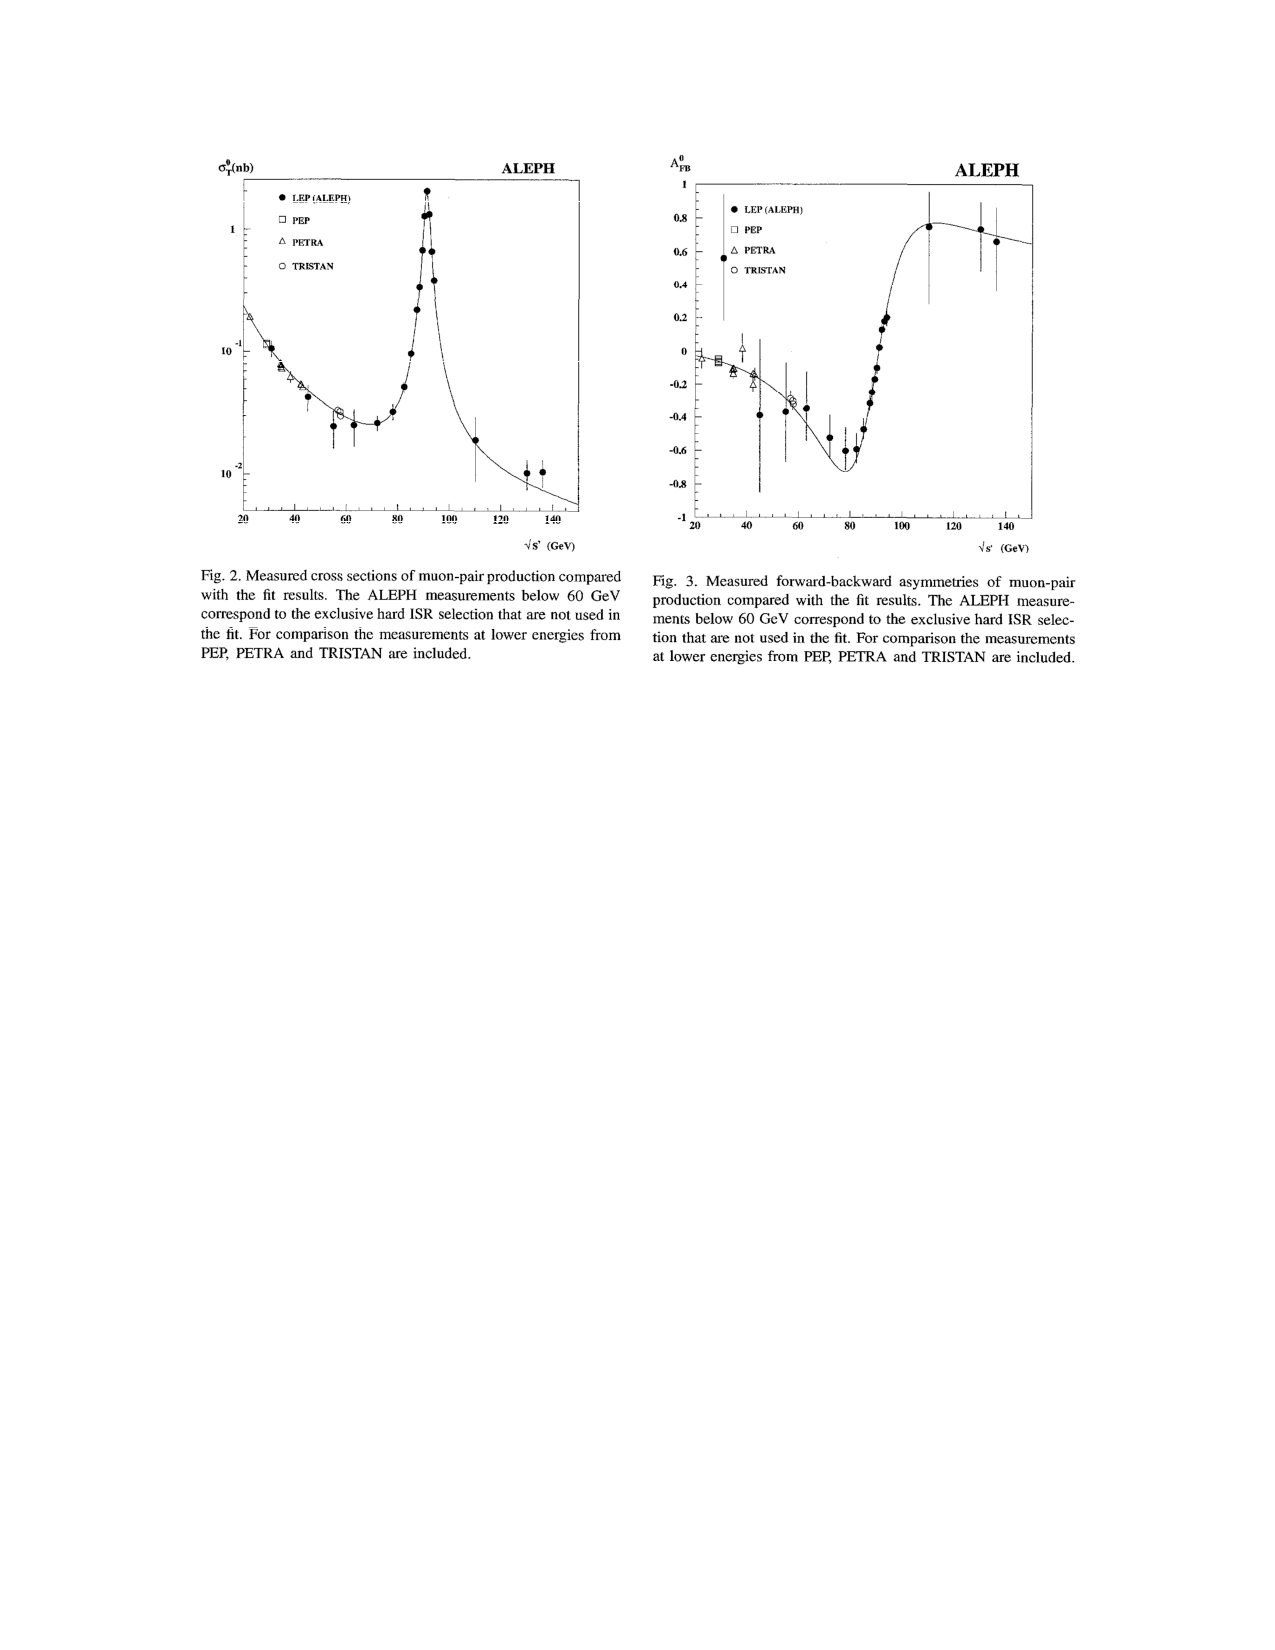
\includegraphics[width=0.8\textwidth]{aleph.pdf}
    \caption{Cross section (left) and forward-backward asymmetry of the muons (right) as a function of $\sqrt{s}$ as measured by the ALEPH Collaboration~\cite{ALEPH:1997gvm}.
    \label{fig:aleph}
    }
\end{figure}

\begin{solution}
    
\end{solution}

\item \textbf{$e^+ e^-\to e^+ e^-$ at NLO in QED} (10 points). 

\begin{enumerate}
    \item Draw all the LO and NLO in QED diagrams for $e^+ e^-\to e^+e^-$. 
    How many are there in total?
    \item Use MadGraph to generate the diagrams up to NLO order in QED.
    The MadGraph syntax for this is:
    \begin{verbatim}
MG5_aMC> generate <process> / <excluded particles> [QED]
    \end{verbatim}
    Note that you will have exclude all particles other than the electrons, positrons, and photons, including so-called ``ghost'' particles.
    You may also get a warning that you need to convert the model to python3 with:
    \begin{verbatim}
convert model /usr/local/venv/MG5_aMC/models/loop_qcd_qed_sm
    \end{verbatim}
    If they don't match up to what you drew, which additional diagrams does MadGraph automatically include and why?
\end{enumerate}

\begin{solution}
    
\end{solution}

\end{enumerate}

\bibliographystyle{cms_unsrt}
\bibliography{main}
\appendix
\section{Reference Formulae}
\label{sec:formulae}

\clearpage
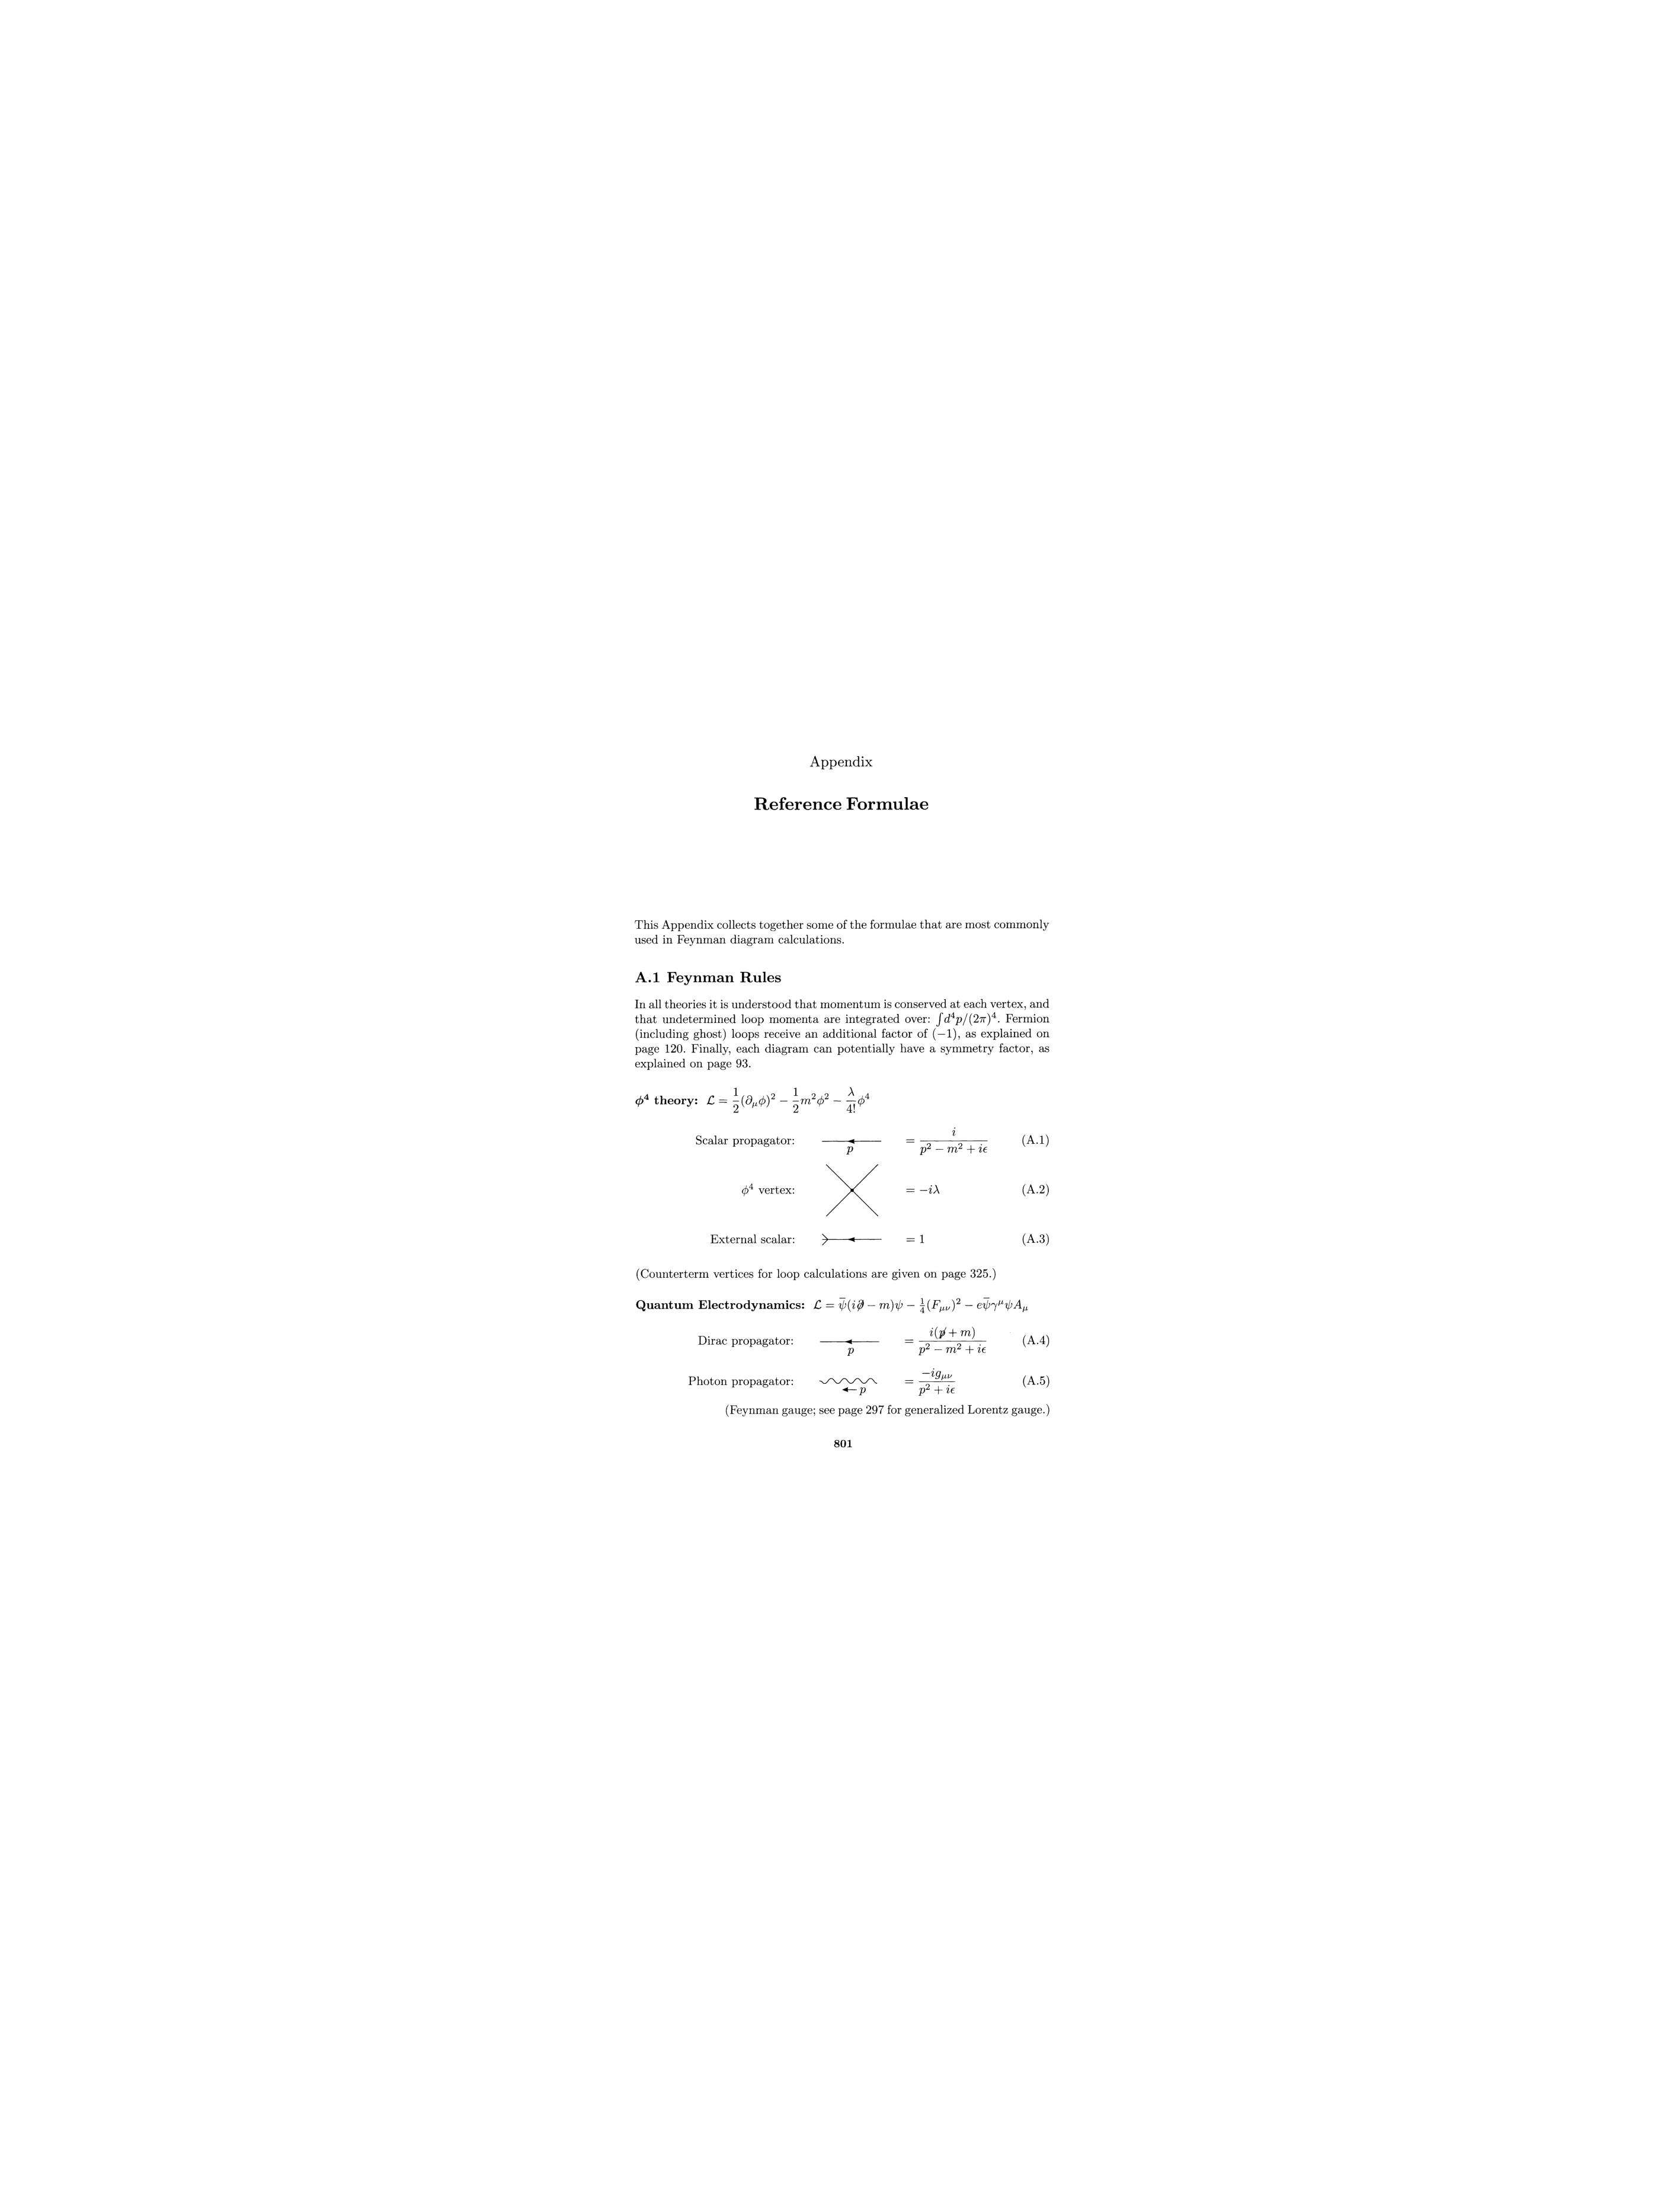
\includepdf[pages=-]{appendix.pdf}
\end{document}